\begin{figure}[h]
	\centering
	\label{fig:loss}
	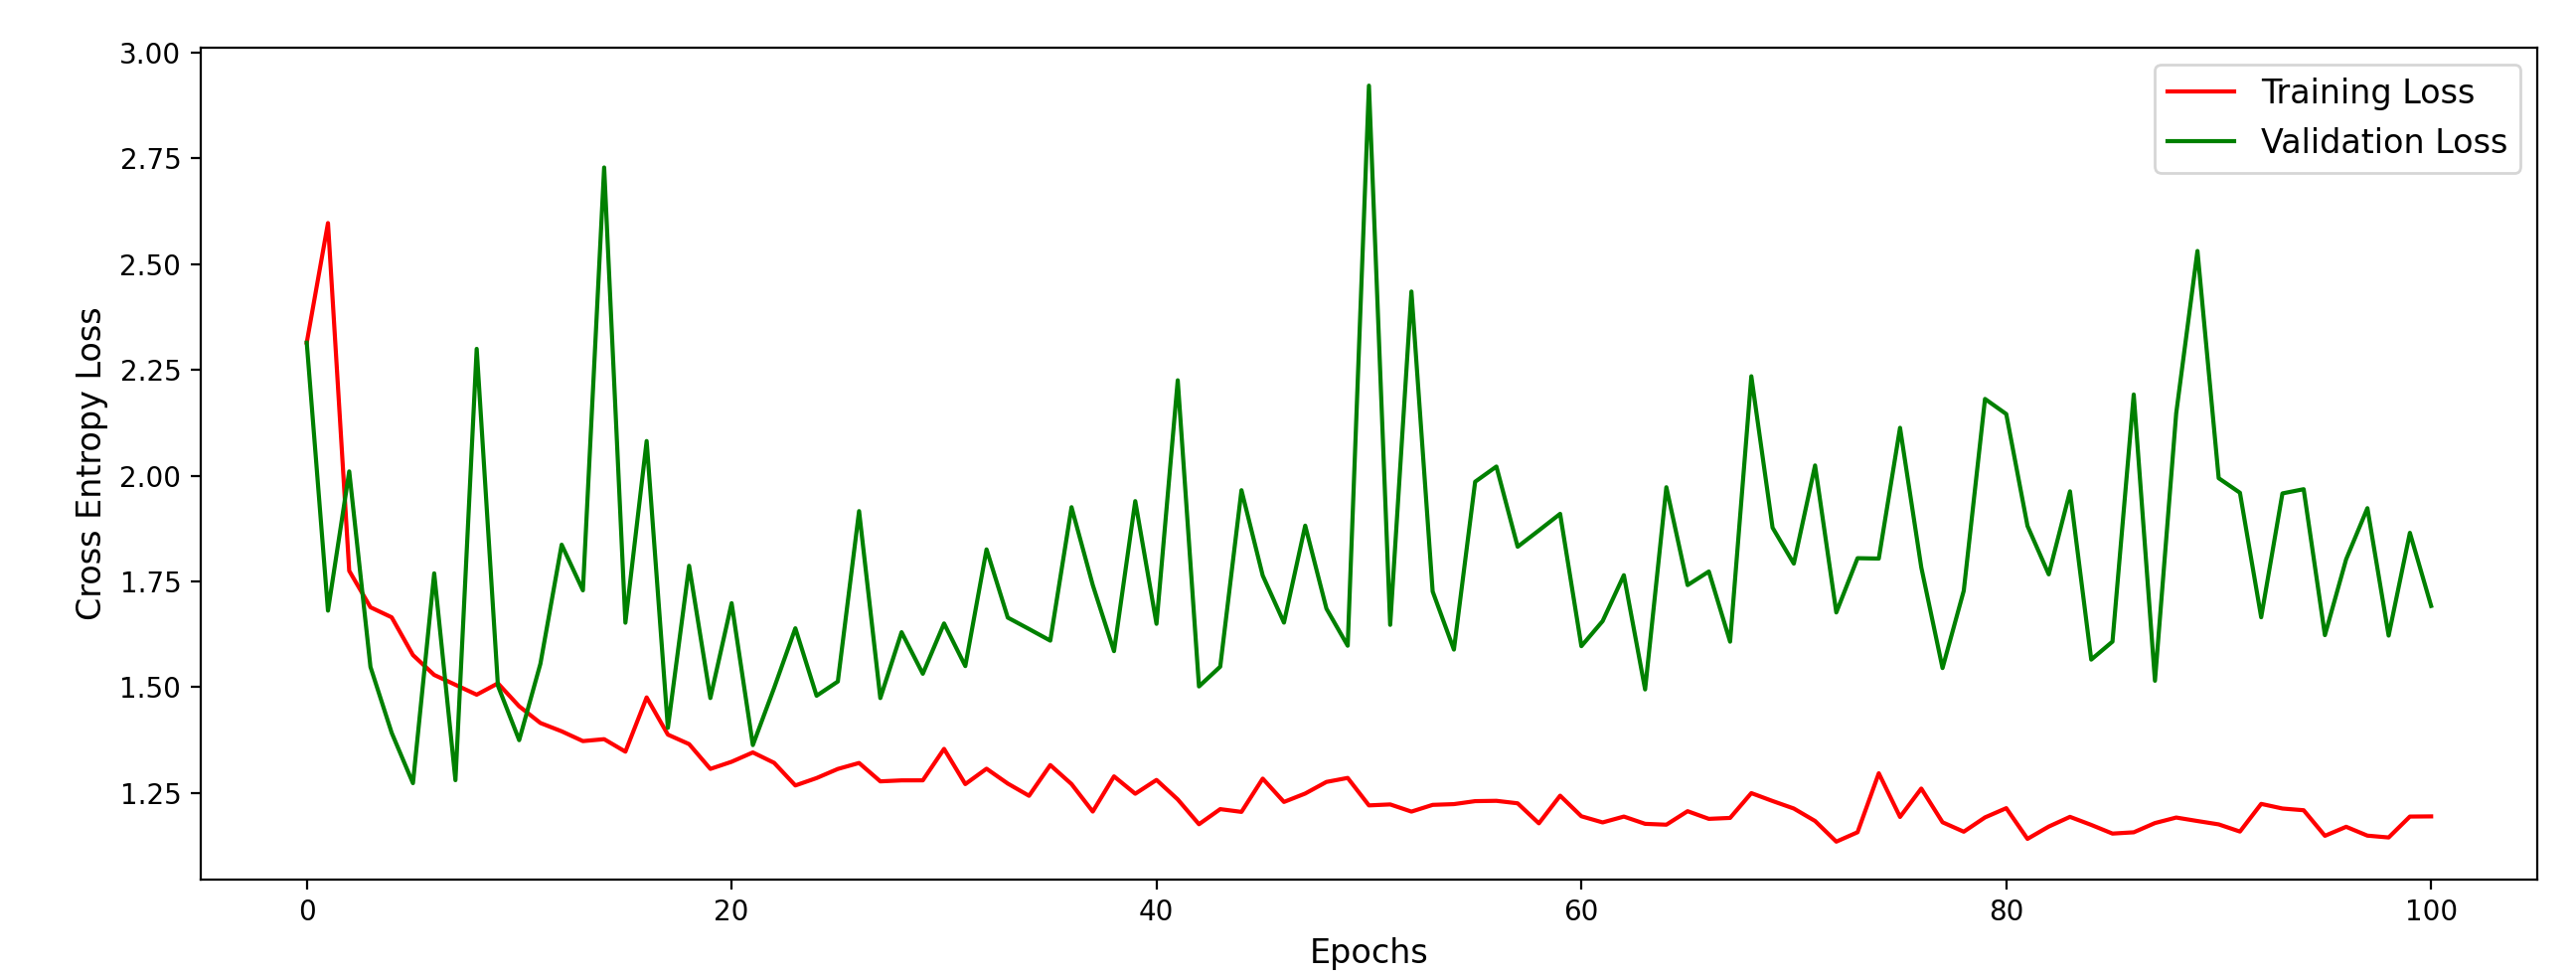
\includegraphics[width=1.0\textwidth]{./images/loss.png}
	\caption{Training/Validation Loss/Accuracy over 100 Epochs}
\end{figure}

\begin{figure}[h]
	\centering
	\label{fig:acc}
	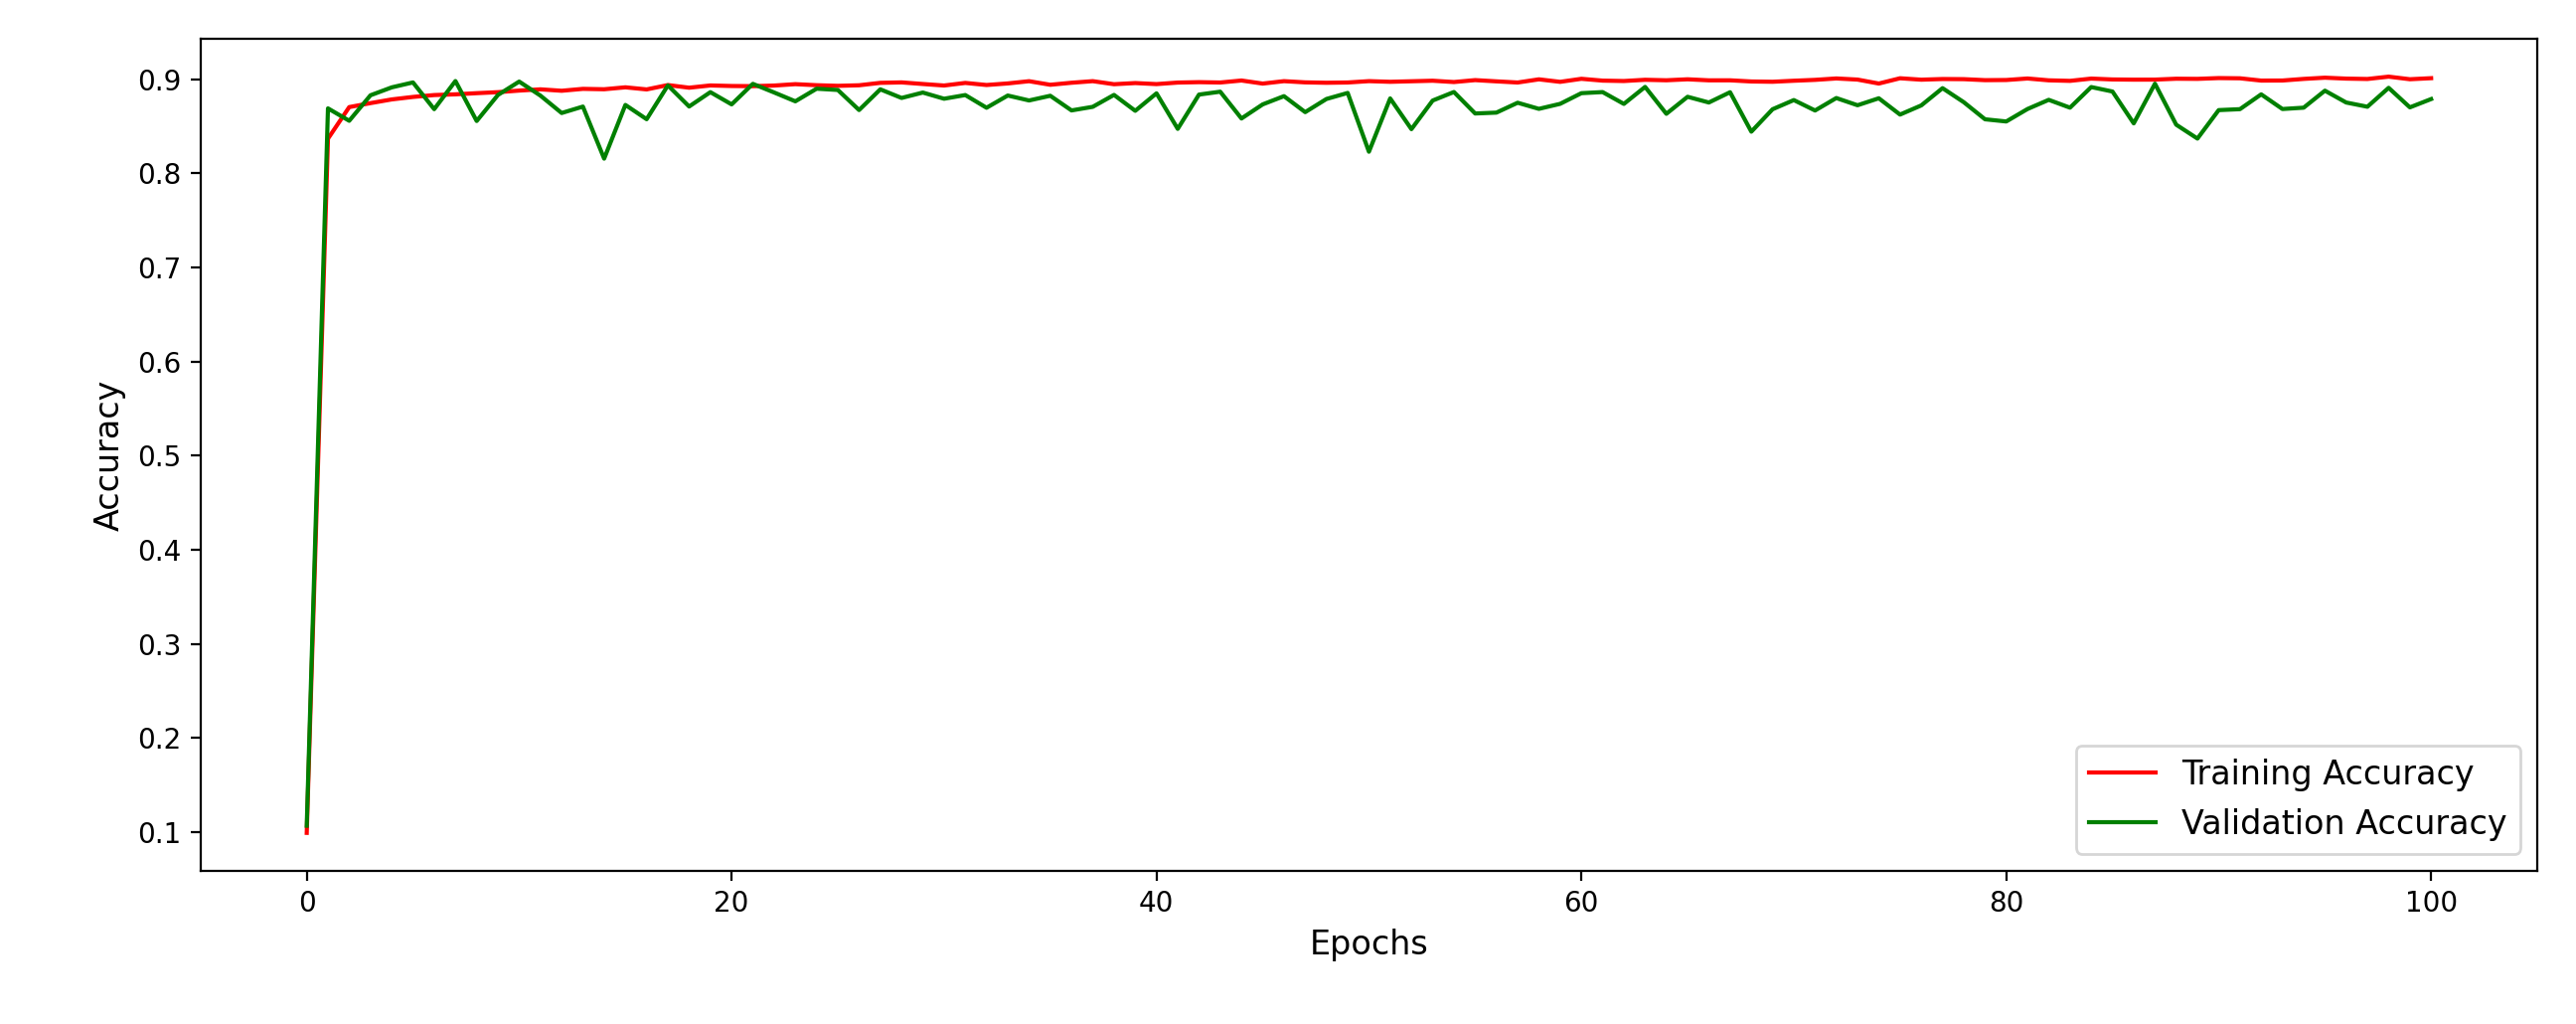
\includegraphics[width=1.0\textwidth]{./images/acc.png}
	\caption{Training/Validation Accuracy over 100 Epochs}
\end{figure}
\section{Softmax Regression}

\subsection{Background}
Firstly, we perform softmax regression on a single-layer neural network (i.e.
input layer directly connects to output layer). Given an input $x^{(n)}$ and $c$
possible classes, softmax regression will output a vector $y^{(n)}$, where each
element, $y^{(n)}_k$ represents the probability that $x^{(n)}$ is in class $k$.

\begin{equation*}
	\begin{aligned}
		y^{(n)}_k & = \text{softmax}(a^{(n)}_k)_ =
		\frac{e^{a^{(n)}_k}}{\sum_{j=1}^{N} e^{a^{(n)}_j}} \\
		a^{(n)}_k & = w^\top_k x^{(n)}
	\end{aligned}
\end{equation*}

Here, the softmax activation function generalizes the logistic activation
function for multiple classes. Now for \textit{softmax regression}, we use a
one-hot encoding for our targets. Together, we can calculate loss via the
cross-entropy cost function defined as

\begin{equation*}
	E = - \sum_k \sum_{k = 1}^c t^{(n)}_k \ln \left( y^{(n)}_k \right)
\end{equation*}

and its corresponding gradient

\begin{equation*}
	-\frac{\partial E^n(w)}{\partial w_{j k}}=\left(t_k^{(n)}-y_k^{(n)}\right) x_j^n
\end{equation*}

The above equations can be combined to implement the following delta rule to
update the weights over each epoch.

\begin{equation*}
	\begin{aligned}
		\delta_j & = (t_j^{(n)}-y_j^{(n)})         & \text{ for output unit } j \\
		\delta_j & = g'(a_j)\sum_k \delta_k w_{jk} & \text{ for hidden unit } j
	\end{aligned}
\end{equation*}

In pseudocode, we have

\begin{algorithm}
	\caption{Stochastic Gradient Descent}
	\begin{algorithmic}
		\State $w \gets 0$
		\For{$t = 1$ to $M$}
		\State Randomize the order of the indices into the training set
		\For{$j = 1$ to $N$ in steps of B}
		\State start = $j$
		\State end = $j$ + B
		\State $w_{t + 1} = w_t - \alpha \sum_{n = \text{start}}^{end} \nabla
			E^{(n)}(w) $
		\EndFor
		\EndFor
	\end{algorithmic}
\end{algorithm}

\subsection{Performance}

In a single layer neural network as defined in \texttt{./config\_4.yaml}, we
obtain the following results using softmax regression over 100 epochs. Below we
plot loss versus epochs~\cref{fig:loss} and accuracy versus epochs~\cref{fig:acc}.
